\subsection{Darfur is Dying}\subparagraph{}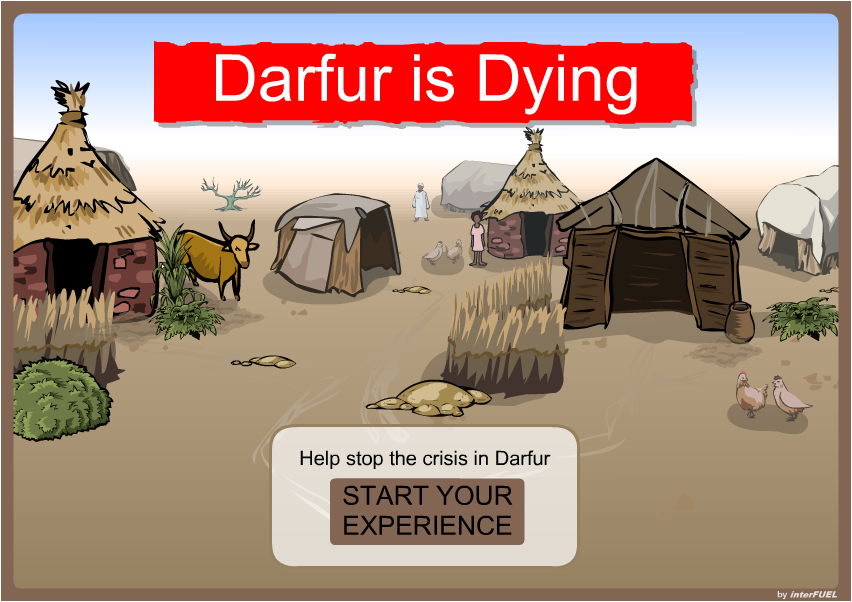
\includegraphics[width = \textwidth]{img/darfur_title.png}\subparagraph{URL}\url{http://www.darfurisdying.com/}\subparagraph{Description}Darfur is Dying, developed by mtvU, is a flash-based game released in April of 2006. The game consists of two main sections. In the first section, players must select a member of a Darfuri refugee; the family consists of a male, female, and several children. Once the player has chosen, the player must guide the refugee to a well using only compass and distance directions, while attempting to avoid Janjaweed militia patrols in trucks. If the player is caught, the game describes the fate of the refugee, and the player is prompted to select another refugee. Once the player has made it to the well, the player must return through the same section to their encampment, but lose water during their journey. Once they have returned to the encampment, the player enters a top-down strategy-like game simulation; they can use the water they have retrieved to grow crops and keep the encampment in good condition. However, if they run out of water, they will need to return to the first section and make the well run again. The goal of the game is to keep the encampment alive for 7 days. In addition, the community is constantly under threat from attacks from the militia; if the militia attacks, the encampment is lost, and the player must start again. The player can prevent attacks from the militia by participating in various viral and advocacy campaign tactics, such as inviting their friends to play, posting on social media, or writing to government officials. \subparagraph{Educational Content}education!\subparagraph{}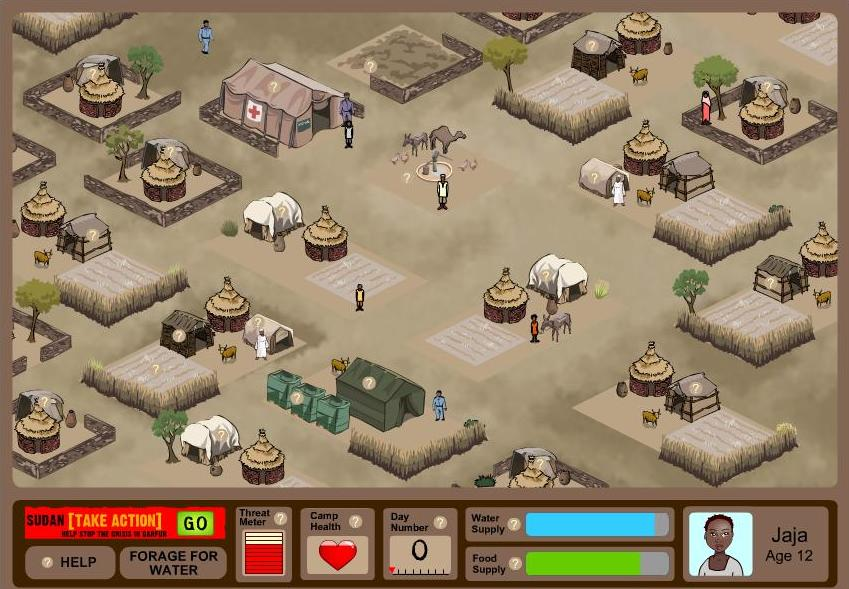
\includegraphics[width = \textwidth]{img/darfur_screen1.jpg}\newpage\subsection{Light Bot}\subparagraph{}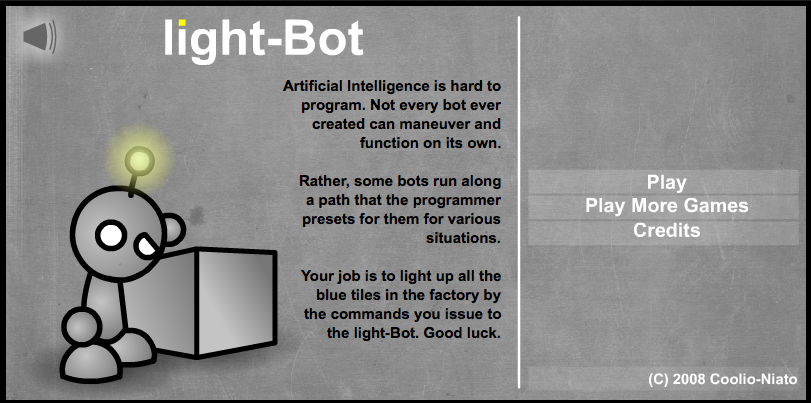
\includegraphics[width = \textwidth]{img/lightbot_title.png}\subparagraph{URL}\url{http://armorgames.com/play/2205/light-bot}\subparagraph{Description}Light Bot, made by Danny Yaroslavski, is a programming and robotics puzzle game. It was originally a flash game, but has since been ported to iOS and Android. Players assume control of a robot on a grid of varying sizes and orientations. Each grid square can also have a height. The robot has the ability to move forward, turn left or right, jump up one level or down one level, and turn a square "on." The robot also has the ability to call "functions," where the robot can execute sequences of events and repeat functions several times or indefinitely. The goal of the robot is to navigate to all of the blue squares and turn them "on" to a yellow state. The robot can do this in any order and using any sequence they like, so long as it fits within the provided instruction spaces. There are 40 levels to the game, ranging from the simple to extremely difficult.\subparagraph{Educational Content}education!\subparagraph{}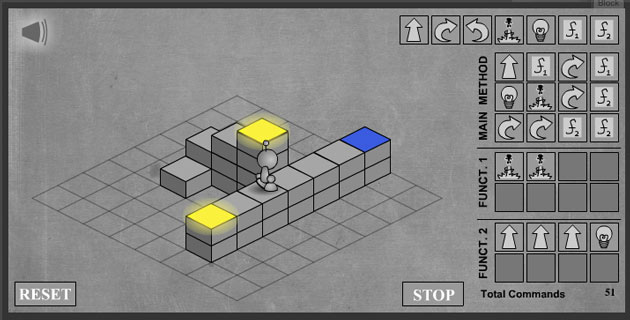
\includegraphics[width = \textwidth]{img/lightbot_screen.jpg}\newpage\subsection{The Incredible Machine}\subparagraph{}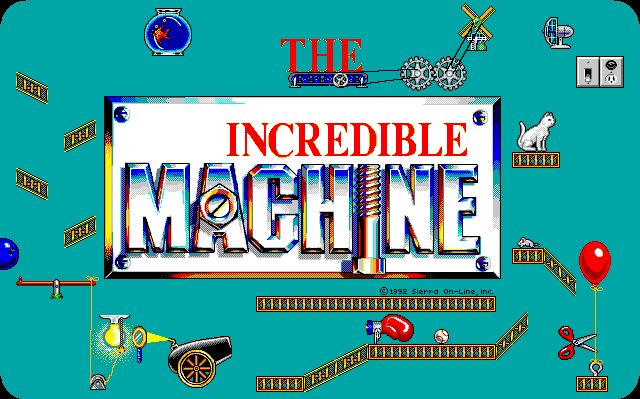
\includegraphics[width = \textwidth]{img/machine_title.png}\subparagraph{URL}\url{http://www.classicdosgames.com/online/timdemo.html}\subparagraph{Description}incredible machine!\subparagraph{Educational Content}education!\subparagraph{}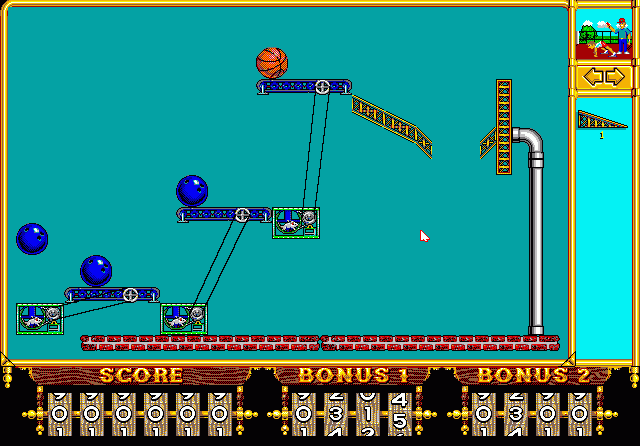
\includegraphics[width = \textwidth]{img/machine_screen.png}\newpage\subsection{Howling Dogs}\subparagraph{}
\includegraphics[width = \textwidth]{img/dogs_title.jpg}\subparagraph{URL}\url{http://aliendovecote.com/uploads/twine/howling%20dogs.html#2m}\subparagraph{Description}An awesome, awesome Twine game\subparagraph{Educational Content}education!\subparagraph{}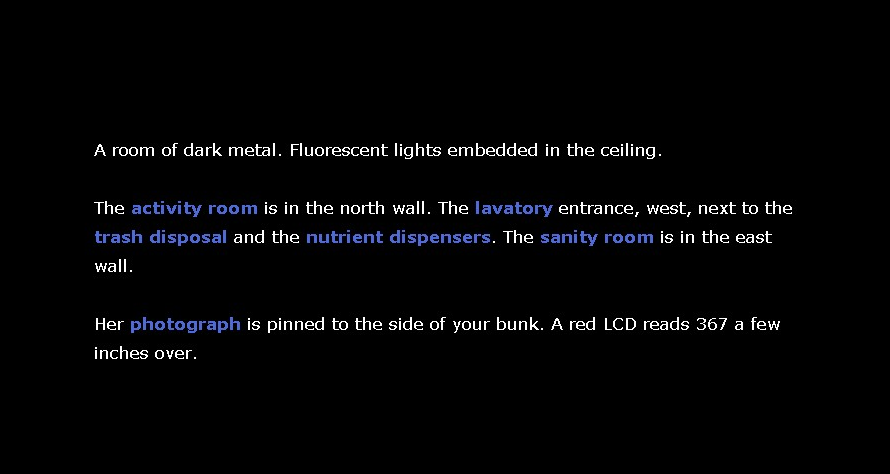
\includegraphics[width = \textwidth]{img/dogs_screen.png}\newpage\subsection{Pandemic 2}\subparagraph{}
\includegraphics[width = \textwidth]{img/pandemic_title.jpg}\subparagraph{URL}\url{http://www.crazymonkeygames.com/Pandemic-2.html#game}\subparagraph{Description}Pandemic 2 is a flash-based strategy game involving infectious diseases, viruses, and bacteria. The player is in charge of designing and mutating an infectious organism, which infects the world population. The objective is to have the infection spread to and kill every human being on the planet, rendering the human race extinct. The virus starts out as being only mildly visible, lethal, and infectious, and can be mutated to more effective versions through "upgrades," received as more humans are infected and die. To combat the spread of the infection, world nations begin to close their borders, set up quarantines, and close off trade routes, cutting off the transmission of the infection to their nation and making it more difficult or nearly impossible for the disease to spread. The player typically alters between the disease upgrade screen and the world monitoring screen, which includes notable headlines and the statuses of the nations. Global high scores are given to players that successfully eliminate the human race in the shortest amount of time.\subparagraph{Educational Content}education!\subparagraph{}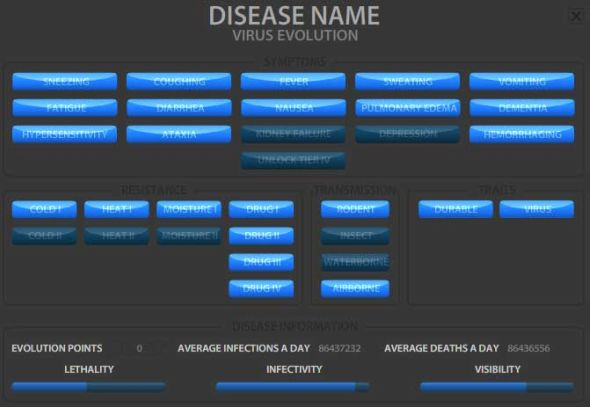
\includegraphics[width = \textwidth]{img/pandemic_screen.jpg}\newpage\subsection{Oregon Trail}\subparagraph{}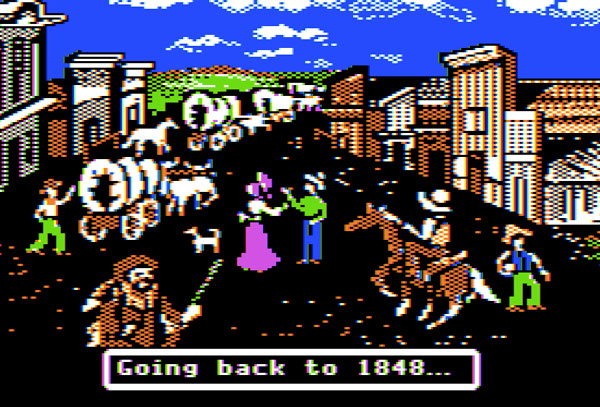
\includegraphics[width = \textwidth]{img/oregon_title.jpg}\subparagraph{URL}\url{http://www.virtualapple.org/oregontraildisk.html}\subparagraph{Description}The Oregon Trail is a series of games detailing the experience of a pioneers traveling the Oregon Trail, a wagon route from the Missouri river to Oregon in 1848. The original game, developed for the Apple II in December of 1971, turned out to be a extremely well received by middle and high school students. In the game, the player first selects an identity which determines how much starting money they have. They then select supplies to buy for their journey; wagons, spare parts, oxen, food, and other supplies. Once they embark on their journey, time passes and food is automatically consumed. Occasionally, players have the chance to hunt, where they can play a simple top-down 2D game to shoot animals that provide food to their party. In addition, numerous events will happen that the player needs to make descisions for, such as a party member falling ill, a wagon part breaking or oxen becoming injured, or needing to cross a river. The player's objective is to travel the entire Oregon Trail with using the minimum amount of resources; the player receives more points at the end for having living party members, items in inventory, and number of dollars, as well as receiving a multiplier if they started the game with less cash.\subparagraph{Educational Content}education!\subparagraph{}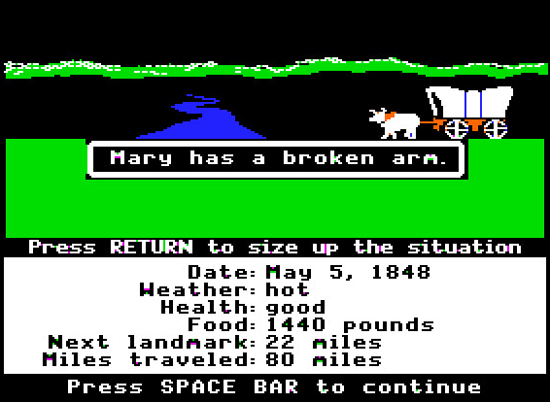
\includegraphics[width = \textwidth]{img/oregon_screen.jpg}\newpage\subsection{Notpron}\subparagraph{}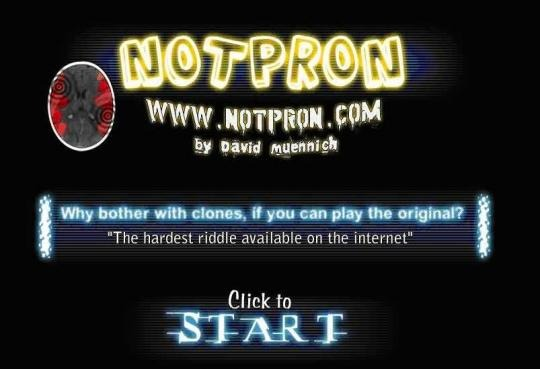
\includegraphics[width = \textwidth]{img/notpron_title.jpeg}\subparagraph{URL}\url{http://notpron.org/notpron/}\subparagraph{Description}An alternate reality game for the browser\subparagraph{Educational Content}education!\subparagraph{}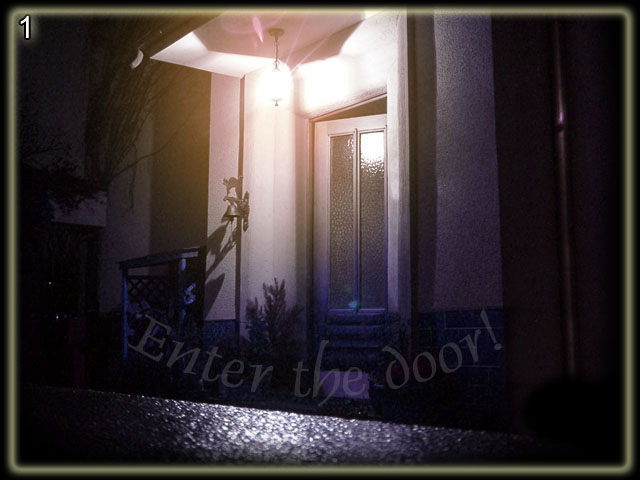
\includegraphics[width = \textwidth]{img/notpron_screen.jpg}\newpage\subsection{Lemmings}\subparagraph{}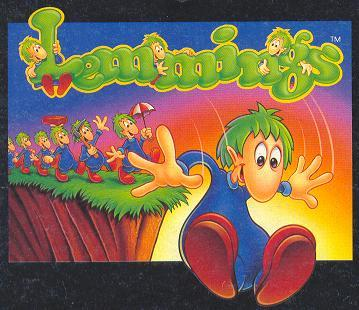
\includegraphics[width = \textwidth]{img/lemmings_title.jpg}\subparagraph{URL}\url{http://www.elizium.nu/scripts/lemmings/}\subparagraph{Description}lemmings!\subparagraph{Educational Content}education!\subparagraph{}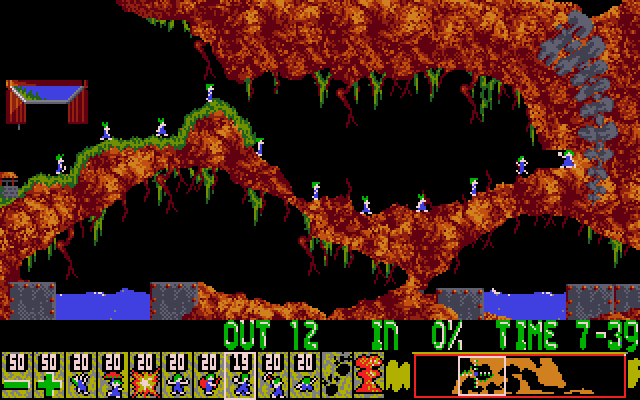
\includegraphics[width = \textwidth]{img/lemmings_screen.jpg}\newpage\subsection{Where in the World is Carmen Sandiego?}\subparagraph{}
\includegraphics[width = \textwidth]{img/carmen_title.jpg}\subparagraph{URL}\url{http://www.xtdos.com/game.php?id=1473}\subparagraph{Description}rockapella\subparagraph{Educational Content}education!\subparagraph{}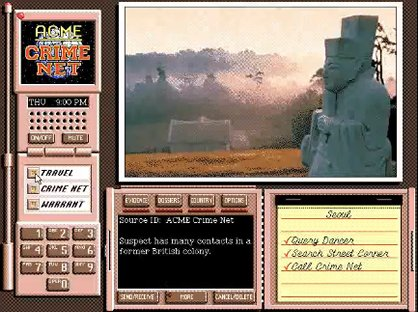
\includegraphics[width = \textwidth]{img/carmen_screen.jpg}\newpage\subsection{Number Munchers}\subparagraph{}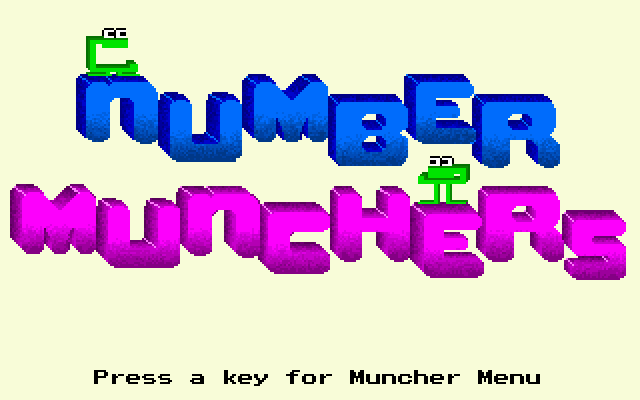
\includegraphics[width = \textwidth]{img/munchers_title.png}\subparagraph{URL}\url{http://wallofgame.com/free-online-games/arcade/988/Number_Munchers.html}\subparagraph{Description}nom nom nom\subparagraph{Educational Content}education!\subparagraph{}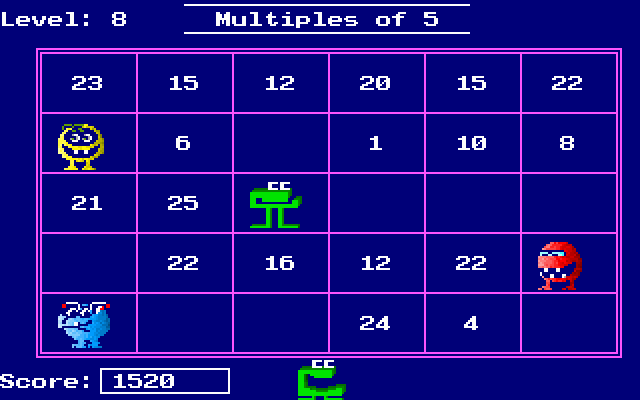
\includegraphics[width = \textwidth]{img/munchers_screen.png}\newpage\subsection{BotLogic}\subparagraph{}
\includegraphics[width = \textwidth]{img/botlogic_title.jpg}\subparagraph{URL}\url{http://botlogic.us/}\subparagraph{Description}dolphin micro\subparagraph{Educational Content}education!\subparagraph{}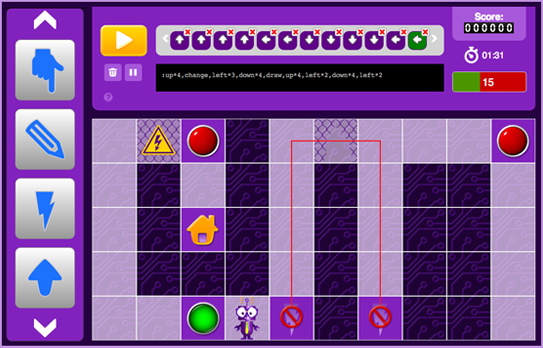
\includegraphics[width = \textwidth]{img/botlogic_screen.png}\newpage\subsection{Math Baseball}\subparagraph{}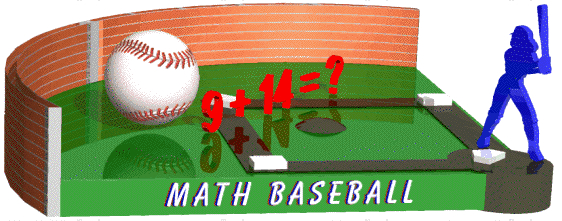
\includegraphics[width = \textwidth]{img/baseball_title.jpg}\subparagraph{URL}\url{http://www.funbrain.com/math/index.html}\subparagraph{Description}how is this even a game\subparagraph{Educational Content}education!\subparagraph{}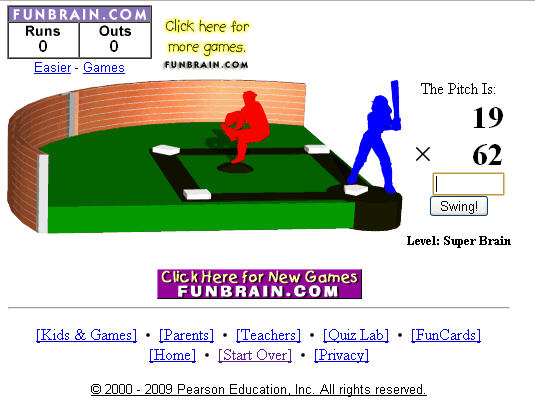
\includegraphics[width = \textwidth]{img/baseball_screen.jpg}\newpage